\chapter{المعالج القبلي (\textenglish{Preprocessor})}

بعد كل المعلومات المتعبة التي تلقّيتها في الفصول حول الجداول، النصوص و المؤشرات، فسنقوم بالتوقف قليلا. لقد تعلّمت أشياء جديدة كثيرة في الفصول السابقة، لن يكون لديّ مانع من نسترجع أنفاسنا قليلا.

هذا الفصل يتحدّث عن المعالج القبلي، هذا البرنامج الّذي يعمل مباشرة قبل الترجمة.\\
لا تخطئ : المعلومات التي به ستكون مهمّة لك. لكنّها ستكون أقل تعقيداً من الّتي تعلّمتها مؤخّراً.

\section{الـ\texttt{include}}

كما شرحت لك  في الفصول الأولى من الكتاب، نجد في الشفرات المصدريّة سطورا خاصّة تسمّى بـ\textbf{توجيهات المعالج القبلي} (\textenglish{Preprocessor directives}).\\
هذه السطور لديها الخاصيّة التالية : تبدأ دائما بالرمز
\InlineCode{\#}.
لذا فمن السهل التعرّف عليها.

التوجيهة الوحيدة التي رأيناها لحدّ الآن هي
\InlineCode{\#include}.\\
هذه التوجيهة تسمح لنا بتضمين محتوى ملف في آخر. قلت لك هذا من قبل.\\
نحن نحتاجها في تضمين الملفات ذات الصيغة
\InlineCode{.h}
كملفات
\InlineCode{.h}
الخاصّة بالمكتبات
(\InlineCode{stdlib.h}، \InlineCode{stdio.h}، \InlineCode{string.h}، \InlineCode{math.h}...)،
و أيضاً ملفات
\InlineCode{.h}
الخاصّة بنا.

لنضمّن ملفاً ذو صيغة
\InlineCode{.h}
موجوداً في نفس المجلّد الذي ثبتنا فيه الـ\textenglish{IDE}
(أي البيئة التطويرية كالـ\textenglish{Code::Blocks}
مثلا)، نستعمل علامات الترتيب
\InlineCode{< >}
كالتالي :

\begin{Csource}
#include <stdlib.h>
\end{Csource}

بينما لتضمين ملفّ
\InlineCode{.h}
موجود في المجلّد الذي به مشروعنا، فسنقوم يذلك باستخدام علامتي الترتيب كالتالي :

\begin{Csource}
#include "myfile.h"
\end{Csource}

في الحقيقة، المعالج القبلي يتمّ تشغيله قبل الترجمة. يبحث في كلّ ملفاتك عن توجيهات المعالج القبلي، تلك الأسطر المشهورة التي تبدأ بـ\InlineCode{\#}.\\
عندما يجد التوجيهة
\InlineCode{\#include}،
يقوم بإدراج محتوى الملفّ في مكان وجود
\InlineCode{\#include}.


افترض أن لديّ ملفّا
\InlineCode{file.c}
يحتوي الشفرة الخاصة بالدوال التي كتبتها، و لدي ملف
\InlineCode{file.h}
يحتوي نماذج الدوال التي هي موجودة بالملف
\InlineCode{file.c}،
يمكن تلخيص ذلك بالمخطط التالي.

\begin{figure}[H]
	\centering
	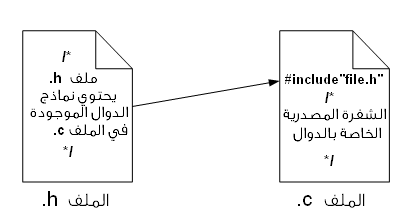
\includegraphics[width=0.8\textwidth]{Chapter_II-5_file-c-file-h}
\end{figure}
كل محتوى الملف
\InlineCode{file.h}
سيتم وضعه داخل الملف
\InlineCode{file.c}
في مكان التوجيهة
\InlineCode{\#include "file.h"}.

تخيّل أن لدينا في الملف
\InlineCode{file.c}
التالي :

\begin{Csource}
#include "file.h"

int myFunction(int something, double stupid)
{
  /* The code of the function */
}
void anotherFunction(int value)
{
  /* The code of the function */
}
\end{Csource}

و في الملف
\InlineCode{file.h} :

\begin{Csource}
int myFunction(int something, double stupid);
void anotherFunction(int value);
\end{Csource}

عندما يمر المعالج القبلي بهذه الشفرة، قبل أن تتم ترجمة الملف
\InlineCode{file.c}،
سيضع كما قلت محتوى الملف
\InlineCode{file.h}
 في الملف
\InlineCode{file.c}.
في النهاية، يعني أن الملف
\InlineCode{file.c}
\textit{قُبَيْل}
الترجمة سيحتوي التالي :

\begin{Csource}
int myFunction(int something, double stupid);
void anotherFunction(int value);

int myFunction(int something, double stupid)
{
  /* The code of the function */
}
void anotherFunction(int value)
{
  /* The code of the function */
}
\end{Csource}

محتوى
\InlineCode{.h}
تمّ إدخاله مكان
\InlineCode{\#include}.

هذا ليس بالأمر المعقد لفهمه، و لعلّ بعض القراء يشكك في أن الأمر يحصل بهذه الطريقة.\\
مع هذه الشروحات الإضافيّة، أتمنّى أنّ يوافقني الجميع.
الـ\InlineCode{\#include}
لا تفعل أي شيء سوى إحضار محتوى ملف و تضمينه في آخر، من المهمّ فهم هذا الأمر جيّدا.

\begin{information}
  إن كنّا قد قررنا وضع النماذج في ملفّات
\InlineCode{.h}
بدل ملفّات
\InlineCode{.c}،
فهذا من المبدأ.
بالطبع، كان بإمكاننا وضع نماذج الدوال في أعلى الملفات
\InlineCode{.c}
بأنفسنا (قد نفعل هذا أحيانا في بعض البرامج الصغيرة)، لكن لأسباب تنظيميّة، من المنصوح به جدّا وضع النماذج في ملفّات
\InlineCode{.h}.
 عندما يكبر برنامجك و يصبح لديك الكثير من ملفّات
\InlineCode{.c}
يعتمدون على نفس
\InlineCode{.h}،
ستكون سعيدا لأنّك لن تظطرّ إلى نسخ و لصق النماذج الخاصّة بنفس الدوال عدّة مرّات !
\end{information}

\section{الـ\texttt{define}}

سنتعرف الآن على توجيهة معالج جديدة و هي
\InlineCode{\#define}.

هذه التوجيهة تسمح بالتصريح عن
\textbf{ثابت معالج قبلي}.
هذا يسمح بإرفاق قيمة بعبارة.\\
إليك مثالا :

\begin{Csource}
#define INITIAL_NUMBER_OF_LIVES 3
\end{Csource}

يجب أن تكتب بالترتيب :

\begin{itemize}
  \item الـ\InlineCode{define}.
  \item الكلمة التي تريد ربط القيمة بها.
  \item قيمة الكلمة.
\end{itemize}

احذر : رغم التشابه (خصوصا في الاسم الذي اعتدنا كتابته بحروف كبيرة)، فهذه مختلفة كثيرا عن الثوابت التي تعلّمناها حتّى الآن، مثل :

\begin{Csource}
const int INITIAL_NUMBER_OF_LIVES = 3;
\end{Csource}

الثوابت تأخذ حيّزا في الذاكرة. حتى و إن لم تتغير قيمتها فإن العدد 3 مخزّن في مكان ما من الذاكرة. هذا ليس هو الحال مع ثوابت المعالج القبلي !

كيف تعمل ؟ في الواقع، الـ\InlineCode{\#define}
تستبدل في شفرتك المصدريّة كلّ الكلمات بقيمتهم الموافقة. هذا تقريبا مثل عمليّة البحث و الاستبدال
(\textenglish{Search / Replace})
الموجودة في برنامج
\textenglish{Word}
مثلا. إذن السطر :

\begin{Csource}
#define INITIAL_NUMBER_OF_LIVES 3
\end{Csource}

يستبدل في الملف كلّ
\InlineCode{INITIAL\_NUMBER\_OF\_LIVES}
بالرقم 3.

هذا مثال على ملف
\InlineCode{.c}
قبل مرور المعالج القبلي :

\begin{Csource}
#define INITIAL_NUMBER_OF_LIVES 3
int main(int argc, char *argv[])
{
	int lives = INITIAL_NUMBER_OF_LIVES;
  /* Code ... */
\end{Csource}
و بعدما يمرّ المعالج القبلي :

\begin{Csource}
int main(int argc, char *argv[])
{
	int lives = 3;
  /* Code ... */
\end{Csource}

قبل الترجمة، كلّ
\InlineCode{\#define}
يتمّ استبدالها بالقيمة الموافقة. المترجم "يرى" الملفّ بعد مرور المعالج القبلي، حيث تكون الاستبدالات قد تمت.

\begin{question}
ما الفائدة بالنسبة للثوابت التي رأيناها حتّى الآن ؟
\end{question}

كما قلت لك، هي لا تأخذ مكانا في الذاكرة. هذا منطقيّ، نظرا لأنّه عند الترجمة لا يتبقّى سوى الأرقام في الشفرة المصدريّة.

توجد فائدة أخرى و هي أنّ الاستبدال يتمّ في كامل الملف حيث توجد
\InlineCode{\#define}.
إن قمت بتعريف ثابت في الذاكرة داخل دالّة، فلن يكون صالحا إلّا داخل تلك الدالّة، ثمّ يتمّ حذفه بعد نهايتها.
بينما بالـنسبة لـ\InlineCode{\#define}
فإنها تُطبّق على كلّ دوال الملف، و هذا قد يكون عمليّا جدّا في بعض الحالات.

هل من مثال واقعيّ لاستخدام
\InlineCode{\#define} ؟\\
هذا ما لن تتأخّر هن فعله. عندما تفتح نافذة في
\textenglish{C}، قد تحتاج إلى تعريف ثوابت المعالج القبلي لتحديد أبعاد النافذة :

\begin{Csource}
#define WINDOW_WIDTH 800
#define WINDOW_HEIGTH 600
\end{Csource}

الفائدة هي أنّه إن أردت تغيير حجم الواجهة (لأنّها تبدو لك صغيرة جدّا)، فيكفي أن تغيّر
\InlineCode{\#define}
و تعيد ترجمة الشفرة.

لاحظ أنّ
\InlineCode{\#define}
تكون عادة في ملفات
\InlineCode{.h}
مع نماذج الدوال (بامكانك أن ترى
\InlineCode{.h}
الخاصّة بالمكتبات مثل
\InlineCode{stdlib.h}،
ستجد الكثير من
\InlineCode{\#define}).\\
\InlineCode{\#define}
إذن هي "مسهّلات وصول"، يمكنك تعديل حجم نافذه عن طريق تعديل
\InlineCode{\#define}
بدل الذهاب للبحث في الدوال عن الموضع الذي تفتح فيه النافذة لتعديل الأبعاد. هذا ربح وقت للمبرمج.

كملخّص، ثوابت المعالج القبلي تسمح بـ"إعداد" برنامجك قبل ترجمته. إنّها أشبه بطريقة إعدادات صغيرة.

\subsection{الـ\texttt{define} من أجل حجم جدول}

نستخدم كثيرا
\InlineCode{\#define}
من أجل تعريف حجم الجداول. نكتب مثلا :

\begin{Csource}
#define MAX_SIZE 1000
int main(int argc, char *argv[])
{
	char string1[MAX_SIZE], string2[MAX_SIZE];
	// ...
\end{Csource}

\begin{question}
  و لكن \dots كنت أعتقد أنّه لا يمكننا وضع متغيّر أو ثابت بين القوسين المربعين أثناء تعريف جدول ؟
\end{question}

نعم هذا صحيح، لكنّ
\InlineCode{MAX\_SIZE}
ليس متغيّرا و لا ثابتا. في الواقع لقد قلت لك، المعالج القبلي يحوّل الملف قبل الترجمة إلى :

\begin{Csource}
int main(int argc, char *argv[])
{
	char string1[1000], string2[1000];
	// ...
\end{Csource}

و هذا شيء صحيح.

بتعريف
\InlineCode{MAX\_SIZE}
بهذه الطريقة، يمكنك استخدامها لإنشاء جداول ذات حجوم محدّدة. إذا صارت في المستقبل غير كافية، فليس عليك سوى تعديل سطر
\InlineCode{\#define}،
إعادة الترجمة، و جداول
\InlineCode{char}
تأخذ القيمة الجديدة الّتي حددتها.

\subsection{الحسابات في الـ\texttt{define}}

من الممكن القيام بحسابات صغيرة في الـ\InlineCode{\#define}.\\
مثلا، هذه الشفرة تنشئ ثابتا
\InlineCode{WINDOW\_WIDTH}،
و آخر
\InlineCode{WINDOW\_HEIGHT}،
ثمّ ثالثا
\InlineCode{PIXELS\_NUMBER}،
الذي يحوي عدد البيكسلز المعروضة داخل النافذة (الحساب بسيط : العرض $\times$ الطول).

\begin{Csource}
#define WINDOW_WIDTH 800
#define WINDOW_HEIGHT 600
#define PIXELS_NUMBER (WINDOW_WIDTH * WINDOW_HEIGHT)
\end{Csource}

قيمة
\InlineCode{PIXELS\_NUMBER}
يتمّ استبدالها قبل الترجمة بالشفرة التالية :
\InlineCode{(WINDOW\_WIDTH * WINDOW\_HEIGHT)}،
أي (800*600)، و تعطينا 480000.
ضع دائما حساباتك بين قوسين كما أفعل من باب الاحتياط لكي تعزل العمليّة.

يمكنك القيام بكل العمليات القاعدية التي تعرفها : جمع (+)، طرح (-)، ضرب (*)، قسمة (/)، ترديد (\%).

\subsection{الثوابت مسبقة التعريف}

بالإضافة إلى الثوابت التي أنت عرّفتها، فإنه توجد ثوابت معرّفة من قِبَل المعالج القبلي.

كل من هذه الثوابت تبدأ و تنتهي برمزي
\textenglish{underscore} \InlineCode{\_}
(تجده في لوحة المفاتيح تحت الرقم 8 أعلى اللوحة بالنسبة للتخطيط
\textenglish{AZERTY}).

\begin{itemize}
  \item \InlineCode{\_\_LINE\_\_} : يعطي رقم السطر الحالي من الشفرة.
  \item \InlineCode{\_\_FILE\_\_} : يعطي اسم الملف الحالي.
  \item \InlineCode{\_\_DATE\_\_} : يعطي تاريخ ترجمة الشفرة.
  \item \InlineCode{\_\_TIME\_\_} : تعطي وقت ترجمة الشفرة.
\end{itemize}

قد تكون هذه الثوابت مفيدة لمعالجة الأخطاء، مثال :

\begin{Csource}
printf("Error in the line n° %d of the file %s\n", __LINE__, __FILE__);
printf("This file has been compiled on %s at %s\n", __DATE__, __TIME__);
\end{Csource}

\begin{Console}
Error in the line n° 9 of the file main.c
This file has been compiled on 13 Jan 2006 at 19:21:10
\end{Console}

\subsection{المعرّفات البسيطة}

إنه من الممكن أن نكتب بكل بساطة :

\begin{Csource}
#define CONSTANT
\end{Csource}

دون إعطاء القيمة.\\
هذا يعني للمعالج القبلي أنّ الكلمة
\InlineCode{CONSTANT}
معرّفة، بكلّ بساطة. ليست لها قيمة لكنّها "موجودة".

\begin{question}
  ما الفائدة من ذلك ؟
\end{question}

القائدة قد لا تبدو واضحة كما كان الأمر في السابق، لكن لهذا فائدة و سنكتشفها بسرعة.

\section{الماكرو (\textenglish{Macro})}

كنا قد رأينا بانه باستعمال الـ\InlineCode{\#define}،
بامكاننا أن نطلب من المعالج القبلي استبدال كلمة بقيمتها في الشفرة بأكملها. مثال :

\begin{Csource}
#define NUMBER 9
\end{Csource}

و الذي يعني أنّ جميع
\InlineCode{NUMBER}
في الشفرة يتمّ استبدالها بـ9. لقد رأينا أنّها تعمل كوظيفة بحث و استبدال يقوم بها المعالج القبلي قبل الترجمة.

لديّ خبر جديد ! في الواقع
\InlineCode{\#define}
أقوى من هذا بكثير. فهي قادرة على الاستبدال بـ\dots شفرة مصدرية بأكملها ! عندما نستخدم
\InlineCode{\#define}
للبحث و استبدال كلمة بشفرة مصدرية نقول أننا أنشأنا
\textbf{ماكرو
(\textenglish{Macro})}.

\subsection{ماكرو بدون معاملات}

هذا مثال عن ماكرو بسيطة :

\begin{Csource}
#define COUCOU() printf("Coucou");
\end{Csource}

الشيء الذي تغيّر هو القوسين الذين أضفناهما بعد الكلمة المفتاحيّة (هنا
\InlineCode{COUCOU()}).
سنرى فائدتهما بعد قليل.

فلنجرب الماكرو داخل الشفرة المصدرية :

\begin{Csource}
#define COUCOU() printf("Coucou");
int main(int argc, char *argv[])
{
  COUCOU()
  return 0;
}
\end{Csource}

\begin{Console}
Coucou
\end{Console}

أعلم أنّ هذا ليس شيئا جديدا حاليّا. لكنّ الّذي عليك فهمه، هو أن الماكرو عبارة عن بضعة أسطر من الشفرة التي يتم استبدالها مباشرة في الشفرة قبل الترجمة.\\
الشفرة التي كتبناها تصبح هكذا قبل الترجمة :

\begin{Csource}
int main(int argc, char *argv[])
{
	printf("Coucou");
	return 0;
}
\end{Csource}

إذا فهمت هذا فقد فهمت مبدأ عمل الماكرو.

\begin{question}
  لكن، هل يمكننا أن نضع سطراً واحدا فقط من الشفرة في كلّ ماكرو ؟
\end{question}

لا، لحسن الحظ يمكنك وضع عدّة أسطر من الشفرة في المرّة. يكفي وضع
\InlineCode{\textbackslash}
قبل كلّ سطر جديد، مثل هذا :

\begin{Csource}
#define TELL_YOUR_STORY() printf("Hello, my name is Brice\n"); \
                          printf("I live at Nice\n"); \
                          printf("I love rice\n");
int main(int argc, char *argv[])
{
	TELL_YOUR_STORY()
	return 0;
}
\end{Csource}

\begin{Console}
Hello, my name is Brice
I live at Nice
I love rice
\end{Console}

كما تلاحظ في
\InlineCode{main}،
أنّ استدعاء الماكرو لا يوضع بعده فاصلة منقوطة في النهاية. في الواقع، لأنها توجيهة خاصة بالمعالج القبلي و لا تحتاج إلى  أن تنتهي بفاصلة منقوطة.

\subsection{ماكرو بالمعاملات}
لحدّ الآن، رأينا كيف نقوم بإنشاء ماكرو بدون معاملات، أي بقوسين فارغين. الفائدة من هذا النوع من الماكرو أنّه يفيد في "اختصار" شفرة طويلة، خاصّة إذا كانت ستتكرّ كثيرا في شفرتك المصدريّة.

لكن الماكرو تصبح مفيدة أكثر عندما نضع لها الأقواس. هذا يعمل تقريبا مثل الدوال :
\begin{Csource}
#define ADULT(age) if (age >= 18) \
                    printf("You are adult\n");
int main(int argc, char *argv[])
{
	ADULT(22)
	return 0;
}
\end{Csource}

\begin{Console}
You are adult
\end{Console}

\begin{information}
يمكننا مثلا إضافة الـ\InlineCode{else}
لكي نُظهر على الشاشة : أنت لست بالغاً
"\textenglish{You are not adult}".
حاول القيام بذلك، الأمر ليس صعبا. لا تنس وضع الشرطة الخلفيّة
\InlineCode{\textbackslash}
قبل السطر الجديد.
\end{information}
مبدأ الماكرو بسيط جدّا :
\begin{Csource}
#define ADULT(age) if (age >= 18) \
                    printf("You are adult\n");
\end{Csource}
نقوم بوضع اسم "متغير" بين القوسين، و الّذي نسميه
\InlineCode{age}.
في كلّ شفرة الماكرو،
\InlineCode{age}
سيتم استبداله بالعدد المحدد عند الاستدعاء (هنا 22).

أي أن الشفرة المصدريّة السابقة بعد مرور المعالج القبلي مباشرة تصبح هكذا :
\begin{Csource}
int main(int argc, char *argv[])
{
	if (22 >= 18)
		printf("You are adult\n");
	return 0;
}
\end{Csource}
تم استبدال السطر الذي يستدعي الماكرو بالشفرة التي تحتويه الماكرو، و تم تعويض "المتغير"
\InlineCode{age}
بقيمته مباشرة في الشفرة المصدريّة للاستبدال.

يمكننا إنشاء ماكرو بعدة معاملات :
\begin{Csource}
#define ADULT(age, name) if (age >= 18)\
			printf("You are adult %s\n", name);
int main(int argc, char *argv[])
{
	ADULT(22, "Maxime")
	return 0;
}
\end{Csource}
هذا كلّ ما يمكننا أن نقوله حول الماكرو و المميزات التي تقدّمها لنا. يمكنك تذكّر أنّه مجرّد استبدال للشفرة المصدرية يمكنه استخدام المعاملات.
\begin{information}
في الواقع، أنت لست بحاجة أن تتعامل كثيراً مع الماكرو، لكن اعلم أن مكتبات معقدة كالـ\textenglish{wxWidgets}
و الـ\textenglish{Qt}
(مكتبات لإنشاء الواجهات الرسوميّة) تستعملان بكثرة الماكرو. لهذا من المستحسن أن تتعلّم كيف تعمل الأمور من الآن كي لا تضيع لاحقا.
\end{information}

\section{الشروط}
أجل : يمكننا أن نستعمل الشروط في لغة المعالج القبلي ! لاحظ كيف تعمل :
\begin{Csource}
#if condition
  /* Code to compile if the condition is true */
#elif condition2
  /* Else, compile this code if the condition2 is true */
#endif
\end{Csource}
الكلمة المفتاحية
\InlineCode{\#if}
تسمح بإدراج شرط معالج قبلي،
\InlineCode{\#elif}
تعني
\InlineCode{else if}.
الأمر يتوقف عندما نضع
\InlineCode{\#endif}،
تلاحظ أنه لا توجد حاضنتان في لغة المعالج القبلي.

الفائدة هي أننا سنتمكن من إجراء
\textbf{ترجمة شرطية
(\textenglish{Conditional compilation})}.\\
في الواقع، إن كان الشرط محققا فإن الشفرة التالية ستتم ترجمتها، و إلّا فسيتم حذفه و لن يكون جزءً من البرنامج النهائي.

\subsection{
\texttt{\#ifdef}
و
\texttt{\#ifndef}
}
سنرى الآن الفائدة من استعمال
\InlineCode{\#define}
لتعريف ثابت دون إعطائه أيّ قيمة، مثلما علّمتك من قبل :
\begin{Csource}
#define CONSTANT
\end{Csource}
في الواقع، يمكننا استعمال الشرط
\InlineCode{\#ifdef}
لنقول "إن كان الثابت معرّفا".
بالنسبة لـ\InlineCode{\#ifndef}،
فهذا يعني "إن كان الثابت غير معرّف".

يمكننا أن نتخيل هذا :
\begin{Csource}
#define WINDOWS
#ifdef WINDOWS
  /* Source code for Windows */
#endif
#ifdef LINUX
  /* Source code for Linux */
#endif
#ifdef MAC
  /* Source code for Mac */
#endif
\end{Csource}
هذا مثال عن برنامج متعدد المنصات
(\textenglish{multi-platform})
للتلاؤم مع النظام مثلا.\\
إذن، يجب من أجل كلّ نظام إعادة ترجمة الشفرة (هذا ليس أمرا سحريّا).
إن كنت في
\textenglish{Windows}
فستكتب
\InlineCode{\#define WINDOWS}
في الأعلى و تعيد الترجمة.\\
إن أردت الترجمة لـ\textenglish{Linux}
فسيكون عليك تغيير
\InlineCode{\#define}
لوضع
\InlineCode{\#define LINUX}
و تعيد الترجمة. هذه المرّة الجزء الخاصّ بـ\textenglish{Linux}
الّذي ستتمّ ترجمته أمّا باقي الشروط فلن تكون محققة يعني أنه سيتم تجاهلها.

\subsection{\texttt{\#ifndef} لتفادي التضمينات اللامنتهية}
\InlineCode{\#ifndef}
مهمّمة جدّا في الملفّات
\InlineCode{.h}
لتجنّب "التضمينات اللامنتهية".
\begin{question}
  ماذا يعني التضمين اللامنتهي ؟
\end{question}
هذا أمر بسيط، تخيل أن لدينا ملفأً
\InlineCode{A.h}
و ملفأً
\InlineCode{B.h}،
الملف
\InlineCode{A.h}
يحتوي
\InlineCode{\#include}
للملف
\InlineCode{B.h}.
إذا فالملف
\InlineCode{B.h}
مضمّن الآن بـ\InlineCode{A.h}.\\
و هنا يبدأ المشكل، تخيّل أن الملف
\InlineCode{B.h}
يحتوي نفسه على
\InlineCode{\#include}
للملف
\InlineCode{A.h} !
هذا يحدث أحيانا في البرمجة ! يعني أن الملف الأول بحاجة إلى الثاني و الثاني بحاجة إلى الأول أيضا.

إن فكّرنا قليلا، فسنعرف أنّ هذا ما سيحصل :
\begin{itemize}
  \item  الحاسوب يقرأ
\InlineCode{A.h}
و يجد بأن عليه تضمين
\InlineCode{B.h}.
  \item يقوم بقراءة
\InlineCode{B.h}
فيجد بأن عليه تضمين
\InlineCode{A.h}.
  \item  يضمّن
\InlineCode{A.h}
في
\InlineCode{B.h}،
لكن داخل
\InlineCode{A.h}
يجد بأنّه يحتاج إلى تضمين
\InlineCode{B.h} !
  \item يكرّر، يرى أنّ
\InlineCode{B.h}
و يجد أنّه يجب عليه تضمين
\InlineCode{A.h}.
  \item إلخ.
\end{itemize}

قد تظنّ أنّ هذا الأمر لا نهاية له !\\
في الحقيقة، من كثرة التضمينات، سيتوقّف المعالج القبلي قائلا "لقد سئمت من التضمينات !" و هذا ما يعطّل الترجمة.

كيف السبيل لوقف هذا الكابوس المريع ؟ إليك الحيلة. أطلب منك فعل هذا في
\textbf{كلّ ملفّات
\InlineCode{.h}
الخاصّة بك} بدون استثناء :

\begin{Csource}
#ifndef DEF_FILENAME // If the constant has not been defined, the file then has never been included
#define DEF_FILENAME // We define the constant so the file will not be included the next time

/* Content of your file .h (other #include, prototypes, #define...) */

#endif
\end{Csource}

أي أننا نضع كل محتوى الملف
\InlineCode{.h}
(بما في ذلك
\InlineCode{\#include}،
النماذج،
\InlineCode{\#define})
بين الـ\InlineCode{\#ifndef}
و الـ\InlineCode{\#endif}.

هل فهمت كيف تعمل الشفرة ؟ أوّل مرّة رأيت هذه التقنيّة كنت مشوّشا كثيرا : سأحاول أن أشرح.

تخيل أن الملف
\InlineCode{.h}
يتم تضمينه للمرة الأولى، سيقرأ الحاسوب الشرط "إذا كان الثابت
\InlineCode{DEF\_FILENAME}
لم يتم تعريفه". بما أنه يتمّ قرائة الملف للمرة الأولى، فإن الثابت لم يتم تعريفه بعد، فسيقوم المعالج القبلي بالدخول إلى داخل
\InlineCode{if}.

أوّل تعليمة سيجدها هي :

\begin{Csource}
#define DEF_FILENAME
\end{Csource}

الآن لقد تم تعريف الثابت. في المرّة القادمة التي يتم فيها تضمين الملف، لن يكون الشرط فيها صحيحا و لهذا لن نخاطر بإعادة تضمين الملف من جديد.

يمكنك تسمية اسم الثابت كما تريد، أنا اعتدت على تسميته
\InlineCode{DEF\_FILENAME}.

الشيء الأهمّ، و الّذي أتمنّى أنّك فهمته جيّدا، هو أن تغيّر اسم الثابت من ملف
\InlineCode{.h}
إلى آخر. يجب ألّا يكون نفس الثابت في كلّ ملفّات
\InlineCode{.h}،
و إلا فلن تتم قراءة سوى أول ملف
\InlineCode{.h}
و الباقية سيتم تجاهلها !\\
إذا فلتغيّر
\InlineCode{FILENAME}
إلى اسم الملف الحالي.
\begin{information}
أنصحك بإلقاء نظرة على
\InlineCode{.h}
الخاصّة بالمكتبات القياسيّة المتواجدة في حاسوبك، سترى بأنها
كلها
مكتوبة بنفس المبدأ
(\InlineCode{\#ifndef}
في البداية و
\InlineCode{\#endif}
في النهاية). هذا يضمن عدم إمكانيّة حصول تضمينات لامنتهية.
\end{information}

\section*{ملخّص}
\begin{itemize}
  \item المعالج القبلي هو برنامج يحلّل الشفرة المصدريّة، و يقوم بإجراء تغييرات علىها قبل الترجمة.
  \item تعليمة المعالج القبلي
\InlineCode{\#include}
تسمح بإدراج محتوى ملف آخر.
  \item تعليمة
\InlineCode{\#define}
تسمح بتعريف ثابت معالج قبلي. يتم استبدال كلمة مفتاحيّة بقيمة في الشفرة المصدريّة.
  \item الماكرو هي مجموعة أسطر من الشفرة الجاهزة معرّفة بالـ\InlineCode{\#define}.
يمكنها أن تقبل معاملات.
  \item من الممكن كتابة شروط في لغة المعالج القبلي لاختيار ما يجب ترجمته، نستعمل عادة
\InlineCode{\#if}،
\InlineCode{\#elif}
و
\InlineCode{\#endif}.
  \item لنتجنب أنّ ملفّاً
\InlineCode{.h}
يتمّ تضمينه عددا لامنتهيا من المرّات، نحميه بمجموعة من ثوابت المعالج القبلي و الشروط. كلّ ملفّاتك
\InlineCode{.h}
المستقبليّة يجب حمايتها بهذه الطريقة.
\end{itemize}
